% !TeX TXS-program:compile = txs:///lualatex

\documentclass[a4paper,11pt]{article}
\usepackage[revgoku]{cp-base}
\graphicspath{{./graphics/}}
%variables
\donnees[%
	classe=1\up{ère} 2M2,matiere={[SPÉ.MATHS]},typedoc=CHAP,numdoc=3,mois=Novembre,annee=2021
]

%formatage
\author{Pierquet}
\title{\nomfichier}
\hypersetup{pdfauthor={Pierquet},pdftitle={\nomfichier},allbordercolors=white,pdfborder=0 0 0,pdfstartview=FitH}
%fancy
\lhead{\entete{\matiere}}
\chead{\entete{\lycee}}
\rhead{\entete{\classe{} - \mois{} \annee}}
%\rhead{\entete{\classe{} - Chapitre }}
\lfoot{\pied{\matiere}}
\cfoot{\logolycee{}}
\rfoot{\pied{\numeropagetot}}

\begin{document}

\pagestyle{fancy}

\part{CH03 - Droites et fonctions affines - Exercices (Correction)}

\smallskip

\exonum{0}%exo1

\begin{enumerate}
	\item La droite $(d)$ est croissante car sa pente ($m=1,5$) est strictement positive.
	\item Le point $A(1~;~7)$ appartient à $(d)$ car $1,5 \times 1 + 5,5 = 7$.
	\item Le point $B(a~;~8)$ appartient à $(d)$ si et seulement si $1,5 \times a+5,5=8$. On résout et on obtient $a=\dfrac53$.
	\item Le point $C(3,5~;~11,5)$ n'appartient pas à $(d)$ car $1,5 \times 3,5 + 5,5 = 10,75 \neq 11,5$.
\end{enumerate}

\medskip

\exonum{1}%exo2


\begin{enumerate}
	\item $f_1(x)=4x-8$ :
	\begin{itemize}
		\item est croissante car $m=4 > 0$ ;
		\item s'annule en $x=2$ ;
		\item est de signe $\ominus0\oplus$.
	\end{itemize}
	\item $f_2(x)=-x+5$ :
	\begin{itemize}
		\item est décroissante car $m=-1 < 0$ ;
		\item s'annule en $x=5$ ;
		\item est de signe $\oplus0\ominus$.
	\end{itemize}
	\item $f_3(x)=3x+5$ :
	\begin{itemize}
		\item est croissante car $m=3 > 0$ ;
		\item s'annule en $x=-\nicefrac{5}{3}$ ;
		\item est de signe $\ominus0\oplus$.
	\end{itemize}
	\item $f_4(x)=-\dfrac23x+\dfrac14$ :
	\begin{itemize}
		\item est décroissante car $m-\nicefrac{2}{3} < 0$ ;
		\item s'annule en $x=\nicefrac{3}{8}$ ;
		\item est de signe $\oplus0\ominus$.
	\end{itemize}
\end{enumerate}

\medskip

\exonum{1}%exo3

\begin{enumerate}
	\item
	\begin{enumerate}
		\item On place les points $A(-1~;~-1)$, $B(1~;~3)$ et $C(2~;~2)$ :
		\begin{center}
			\begin{tikzpicture}[x=0.7cm,y=0.7cm,xmin=-2,xmax=4,ymin=-2,ymax=4]
				\tgrillep \axestikz* \axextikz*{-2,-1,...,3} \axeytikz*{-2,-1,...,3}
				\clip (\xmin,\ymin) rectangle (\xmax,\ymax) ;
				\draw[ultra thick,red,domain=\xmin:\xmax,samples=2] plot (\x,{2*\x+1}) ;
				\draw[ultra thick,blue,domain=\xmin:\xmax,samples=2] plot (\x,{\x}) ;
				\draw[ultra thick,ForestGreen,domain=\xmin:\xmax,samples=2] plot (\x,{-\x+4}) ;
				\foreach \Point/\Nom/\Pos in {(-1,-1)/A/above left,(1,3)/B/left,(2,2)/C/right}
					\filldraw \Point circle[radius=2pt] node[\Pos] {\Large \point{\Nom}} ;
			\end{tikzpicture}
		\end{center}
		\item On lit -- graphiquement (!) -- que :
		\begin{itemize}
			\item $(AB)$ : $y=2x+1$ ;
			\item $(AC)$ : $y=x$ ;
			\item $(BC)$ : $y=-x+4$.
		\end{itemize}
	\end{enumerate}
	\item Par lectures graphiques :
	\begin{itemize}
		\item $(d_1)$ : $y=-x+2$ ;
		\item $(d_2)$ : $y=3x-1$ ;
		\item $(d_3)$ : $y=y=2$ ;
		\item $(d_4)$ : $y=0,8x-2$ ;
		\item $(d_5)$ : $x=4$ ;
		\item $(d_6)$ : $y=30x-20$ ;
		\item $(d_7)$ : $y=-\tfrac{10}{3}x+80$ ;
		\item $(d_8)$ : $y=4x$.
	\end{itemize}
\end{enumerate}

\medskip

\exonum{2}%exo4

\begin{enumerate}
	\item Par \uline{calculs} :
	\begin{itemize}
		\item $m=\dfrac{DV}{DH}=\dfrac{y_L-y_K}{x_L-x_K}=\dfrac{65,47-15,75}{100,4-10}=0,55$ ;
		\item ainsi $(KL)$ : $y=0,55x+p$ ;
		\item avec $K$, on obtient $0,55 \times 10 + p = 15,75 \Rightarrow p = 15,75 - 0,55 \times 10 = 10,25$.
	\end{itemize}
	Ainsi on obtient $(KL)$ : $y=0,55x+10,25$.
	\item Le point de coordonnées $(50\,;\,37,85)$ n'appartient pas à la droite $(KL)$ car $0,55 \times 50 + 10,25 = 37,74 \neq 37,85$.
\end{enumerate}

\medskip

\exonum{1}%exo5

\begin{enumerate}
	\item
	\begin{enumerate}
		\item Le coefficient directeur de $(AB)$ vaut $m_{(AB)}=\dfrac{y_B-y_A}{x_B-x_A}=\dfrac{8-2}{2-1}=6$.
		\item Le coefficient directeur de la droite $(AC)$ est $m_{(AC)}=\dfrac{y_C-y_A}{x_C-x_A}=\dfrac{26-2}{5-1}=6$.
		\item Une équation de $(AB)$ est $y=6x-4$ (car $p=2-6\times1$).
	\end{enumerate}
	\item On va regarder si $C$ appartient à la droite $(AB)$ : $6 \times 5 - 4 = 26$ $\checkmark$.
	
	Donc les points $A$, $B$ et $C$ sont bien alignés.
\end{enumerate}

\medskip

\exonum{3}%exo6

\begin{enumerate}
	\item Les expressions suivantes sont bien sous forme de produit(s)/quotient(s), donc tds ok :
	\begin{enumerate}
		\item $(x-3)(2x-4)$ :
		\begin{center}
			\begin{tikzpicture}
				\tkzTabInit[]{$x$/0.8,$(x-3)$/0.8,$(2x-4)$/0.8,expr/0.8}{$-\infty$, $2$, $3$, $+\infty$}
				\draw[] (T21) -- (T22) node [midway, right] {$\: m=1 \: \oplus$};
				\draw[] (T22) -- (T23) node [midway, right] {$\: m=2 \: \oplus$};
				\tkzTabLine{,-,t,-,z,+,}
				\tkzTabLine{,-,z,+,t,+,}
				\tkzTabLine{,+,z,-,z,+,}
			\end{tikzpicture}
			
			\smallskip
			
			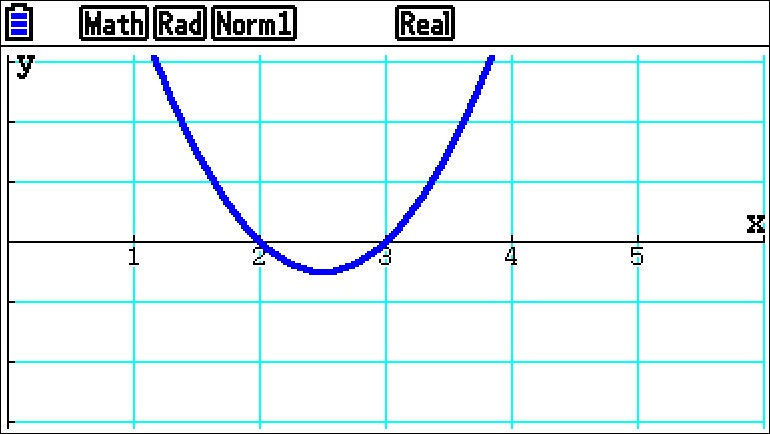
\includegraphics[width=4.5cm]{chap03_corr_exo6_a}
			
			\pagebreak
		\end{center}
		\item $-x(3x+4)$ :
		\begin{center}
			\begin{tikzpicture}
				\tkzTabInit[]{$x$/0.8,$-x$/0.8,$(3x+4)$/0.8,expr/0.8}{$-\infty$, $-\nicefrac{4}{3}$, $0$, $+\infty$}
				\draw[] (T21) -- (T22) node [midway, right] {$\: m=-1 \: \ominus$};
				\draw[] (T22) -- (T23) node [midway, right] {$\: m=3 \: \oplus$};
				\tkzTabLine{,+,t,+,z,-,}
				\tkzTabLine{,-,z,+,t,+,}
				\tkzTabLine{,-,z,+,z,-,}
			\end{tikzpicture}
			
			\smallskip
			
			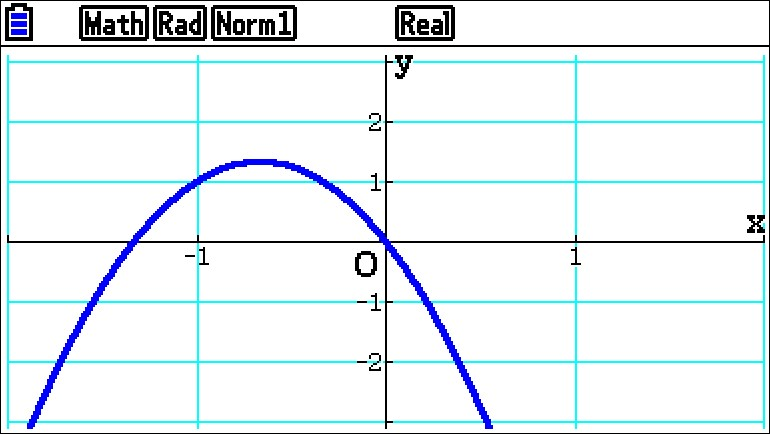
\includegraphics[width=4.5cm]{chap03_corr_exo6_b}
		\end{center}
		\item $(x-2)(x+5)(7-7x)$ :
		\begin{center}
			\begin{tikzpicture}
				\tkzTabInit[espcl=2.5]{$x$/0.8,$(x-2)$/0.8,$(x+5)$/0.8,$(7-7x)$/0.8,expr/0.8}{$-\infty$, $-5$, $1$,$2$,$+\infty$}
				\draw[] (T21) -- (T22) node [midway, right] {$\: m=1 \: \oplus$};
				\draw[] (T22) -- (T23) node [midway, right] {$\: m=1 \: \oplus$};
				\draw[] (T23) -- (T24) node [midway, right] {$\: m=-7 \: \ominus$};
				\tkzTabLine{,-,t,-,t,-,z,+,}
				\tkzTabLine{,-,z,+,t,+,t,+,}
				\tkzTabLine{,+,t,+,z,-,t,-,}
				\tkzTabLine{,+,z,-,z,+,z,-,}
			\end{tikzpicture}
			
			\smallskip
			
			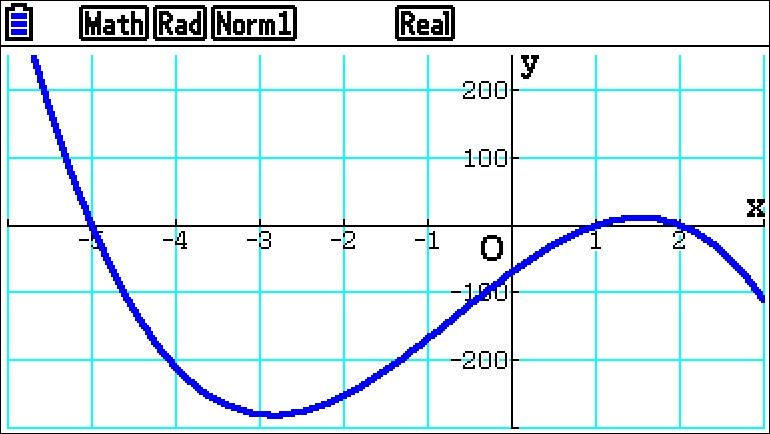
\includegraphics[width=4.5cm]{chap03_corr_exo6_c}
		\end{center}
		\item $\dfrac{2x+1}{(x-5)(x-1)}$ :
		\begin{center}
			\begin{tikzpicture}[double distance=3]
				\tkzTabInit[espcl=2.5]{$x$/0.8,$(2x+1)$/0.8,$(x-5)$/0.8,$(x-1)$/0.8,expr/0.8}{$-\infty$, ${-0,5}$, $1$,$5$,$+\infty$}
				\draw[] (T21) -- (T22) node [midway, right] {$\: m=2 \: \oplus$};
				\draw[] (T22) -- (T23) node [midway, right] {$\: m=1 \: \oplus$};
				\draw[] (T23) -- (T24) node [midway, right] {$\: m=1 \: \oplus$};
				\draw(N31) node [yshift=3pt] {{\scriptsize \red \textsf{D}}};
				\draw(N41) node [yshift=3pt] {{\scriptsize \red \textsf{D}}};
				\tkzTabLine{,-,z,+,t,+,t,+,}
				\tkzTabLine{,-,t,-,t,-,z,+,}
				\tkzTabLine{,-,t,-,z,+,t,+,}
				\tkzTabLine{,-,z,+,d,-,d,+,}
			\end{tikzpicture}
			
			\smallskip
			
			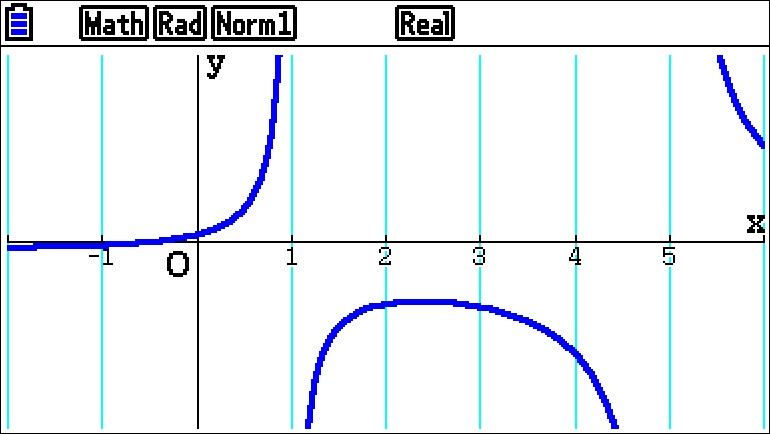
\includegraphics[width=4.5cm]{chap03_corr_exo6_d}
		\end{center}
		
		\pagebreak
		\item $\dfrac{-7(x+2)}{5-2x}$ :
		\begin{center}
			\begin{tikzpicture}[double distance=3]
				\tkzTabInit[]{$x$/0.8,$-7$/0.8,$(x+2)$/0.8,$(5-2x)$/0.8,expr/0.8}{$-\infty$, ${-2}$, ${2,5}$,$+\infty$}
				\draw[] (T22) -- (T23) node [midway, right] {$\: m=1 \: \oplus$};
				\draw[] (T23) -- (T24) node [midway, right] {$\: m=-2 \: \ominus$};
				\draw(N31) node [yshift=3pt] {{\scriptsize \red \textsf{D}}};
				\tkzTabLine{,-,t,-,t,-,}
				\tkzTabLine{,-,z,+,t,+,}
				\tkzTabLine{,+,t,+,z,-,}
				\tkzTabLine{,+,z,-,d,+,}
			\end{tikzpicture}
			
			\smallskip
			
			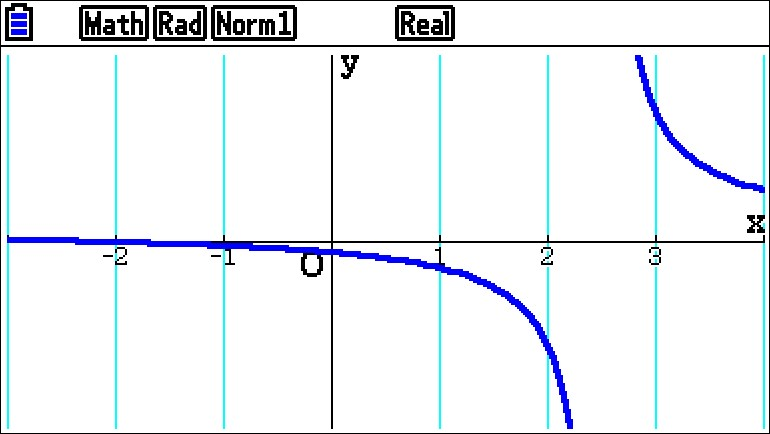
\includegraphics[width=4.5cm]{chap03_corr_exo6_e}
		\end{center}
		\item $\dfrac{x^2+3}{(x-1)(x+4)}$ :
		\begin{center}
			\begin{tikzpicture}[double distance=3]
				\tkzTabInit[]{$x$/0.8,$(x^2+3)$/0.8,$(x-1)$/0.8,$(x+4)$/0.8,expr/0.8}{$-\infty$, ${-4}$, ${1}$,$+\infty$}
				\draw[] (T22) -- (T23) node [midway, right] {$\: m=1 \: \oplus$};
				\draw[] (T23) -- (T24) node [midway, right] {$\: m=1 \: \oplus$};
				\draw(N21) node [yshift=3pt] {{\scriptsize \red \textsf{D}}};
				\draw(N31) node [yshift=3pt] {{\scriptsize \red \textsf{D}}};
				\tkzTabLine{,+,t,+,t,+,}
				\tkzTabLine{,-,t,-,z,+,}
				\tkzTabLine{,-,z,+,t,-,}
				\tkzTabLine{,+,d,-,d,+,}
			\end{tikzpicture}
			
			\smallskip
			
			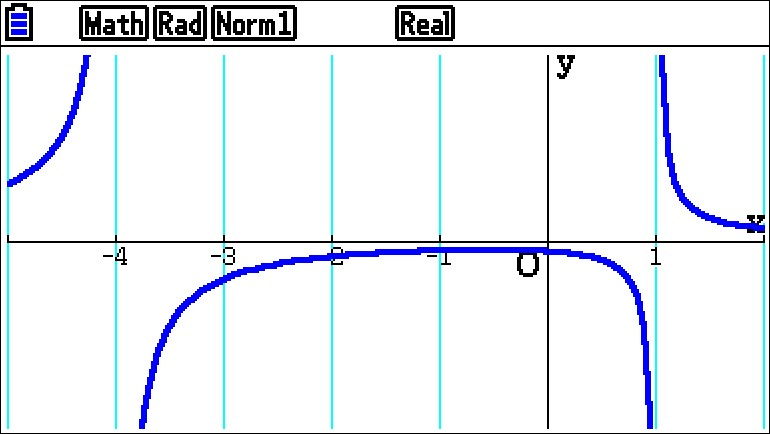
\includegraphics[width=4.5cm]{chap03_corr_exo6_f}
		\end{center}
	\end{enumerate}
	\item On utilise, ci-besoin, les techniques habituelles pour transformer
	\begin{enumerate}
		\item $(x-3)(x-1) -2(x-3)(4x-7) = (x-3)\left[ (x-1)-2(4x-7)\right] = (x-3)(x-1-8x+14)=(x-3)(-7x+13)$ :
		\begin{center}
			\begin{tikzpicture}
				\tkzTabInit[lgt=2.5]{$x$/0.8,$(x-3)$/0.8,$(-7x+13)$/0.8,expr/0.8}{$-\infty$, $\nicefrac{13}{7}$, $3$, $+\infty$}
				\draw[] (T21) -- (T22) node [midway, right] {$\: m=1 \: \oplus$};
				\draw[] (T22) -- (T23) node [midway, right] {$\: m=-7 \: \ominus$};
				\tkzTabLine{,-,t,-,z,+,}
				\tkzTabLine{,+,z,-,t,-,}
				\tkzTabLine{,-,z,+,z,-,}
			\end{tikzpicture}
			
			\smallskip
			
			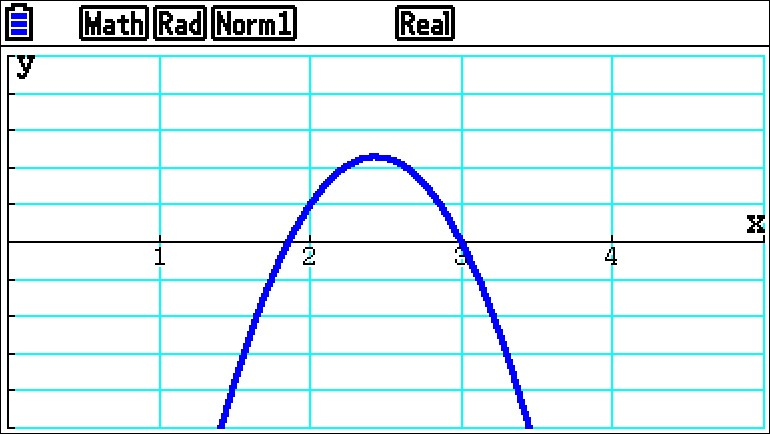
\includegraphics[width=4.5cm]{chap03_corr_exo6_g}
		\end{center}
		
		\pagebreak 
		\item $3-\dfrac{5+x}{7x-13} = \dfrac{3(7x-13)}{7x-13} - \dfrac{5+x}{7x-13} = \dfrac{21x-39-5-x}{7x-13} = \dfrac{20x-44}{7x-13}$ :
		\begin{center}
			\begin{tikzpicture}[double distance=3]
				\tkzTabInit[lgt=2.5]{$x$/0.8,$(20x-44)$/0.8,$(7x-13)$/0.8,expr/0.8}{$-\infty$, $\nicefrac{13}{7}$, $\nicefrac{11}{5}$, $+\infty$}
				\draw[] (T21) -- (T22) node [midway, right] {$\: m=20 \: \oplus$};
				\draw[] (T22) -- (T23) node [midway, right] {$\: m=7 \: \oplus$};
				\draw(N21) node [yshift=3pt] {{\scriptsize \red \textsf{D}}};
				\tkzTabLine{,-,t,-,z,+,}
				\tkzTabLine{,-,z,+,t,+,}
				\tkzTabLine{,+,d,-,z,+,}
			\end{tikzpicture}
			
			\smallskip
			
			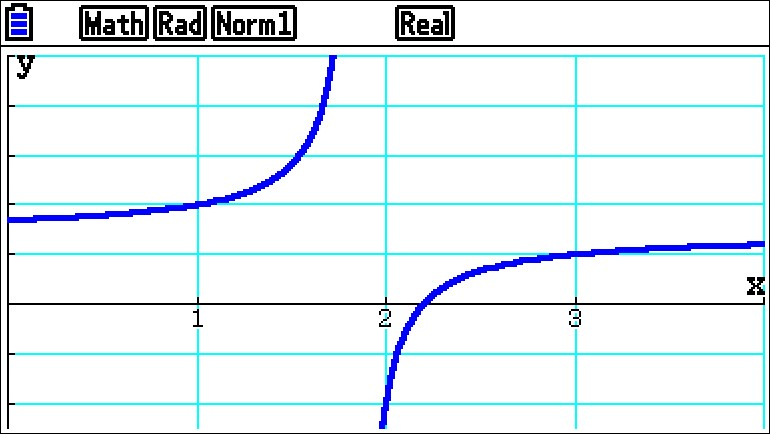
\includegraphics[width=4.5cm]{chap03_corr_exo6_h}
		\end{center}
		\item $x(x+2)(x-3)^2 = x(x+2)(x-3)(x-3)$ :
		\begin{center}
			\begin{tikzpicture}[]
				\tkzTabInit[espcl=2.75]{$x$/0.8,$x$/0.8,$(x+2)$/0.8,$(x-3)$/0.8,$(x-3)$/0.8,expr/0.8}{$-\infty$, ${-2}$, ${0}$,$3$,$+\infty$}
				\draw[] (T21) -- (T22) node [midway, right] {$\: m=1 \: \oplus$};
				\draw[] (T22) -- (T23) node [midway, right] {$\: m=1 \: \oplus$};
				\draw[] (T23) -- (T24) node [midway, right] {$\: m=1 \: \oplus$};
				\draw[] (T24) -- (T25) node [midway, right] {$\: m=1 \: \oplus$};
				\tkzTabLine{,-,t,-,z,+,t,+,}
				\tkzTabLine{,-,z,+,t,+,t,+,}
				\tkzTabLine{,-,t,-,t,-,z,+,}
				\tkzTabLine{,-,t,-,t,-,z,+,}
				\tkzTabLine{,+,z,-,z,+,z,+,}
			\end{tikzpicture}
			
			\smallskip
			
			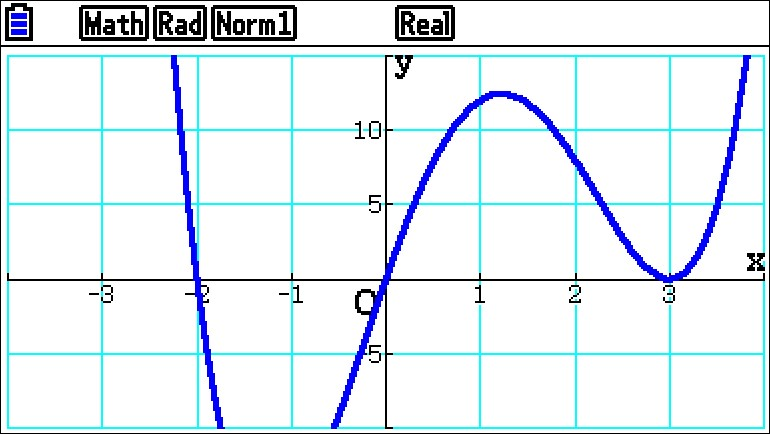
\includegraphics[width=4.5cm]{chap03_corr_exo6_i}
		\end{center}
	\end{enumerate}
\end{enumerate}

\medskip

\exonum{3}%exo7

\begin{enumerate}
	\item On peut résoudre, à l'aide d'un tds :
	\begin{enumerate}
		\item $(x-3)(2x+4) \pg 0$  donne $\mathscr{S} = \intervOF{\strut-\infty}{-2} \cup \intervFO{3}{\strut+\infty}$.
		\item $3x(x+1)(7+x) < 0$ donne $\mathscr{S} = \intervOO{\strut-\infty}{-7} \cup \intervOO{-1}{\strut 0}$.
		\item $\dfrac{x+3}{2x+8} \pp 0$ donne $\mathscr{S} = \intervOF{\strut-4}{-3}$.
		\item $\dfrac{x(x+2)}{x+1} > 0$ donne $\mathscr{S} = \intervOO{\strut-2}{-1} \cup \intervOO{0}{\strut+\infty}$.
	\end{enumerate}
	\item En utilisant les techniques de \textit{transformation}, on transforme pour pouvoir réaliser un tds :
	\begin{enumerate}
		\item $7x+3 \pp 2 \ssi 7x+1 \pp 0$ donne $\mathscr{S} = \intervOO{-\infty}{\strut-\tfrac{1}{7}}$.
		\item $(x+1)(x-2) < (x+1)(4x+5) \ssi (x+1)(x-2)-(x+1)(4x-5) < 0 \ssi (x+1)(x-2-4x-5) < 0$.
		
		Et $(x+1)(-3x-7) < 0$ donne $\mathscr{S} = \intervOO{\strut-\infty}{-\tfrac{7}{3}} \cup \intervOO{-1}{\strut+\infty}$.
		\item $\dfrac{x+1}{x+2} < 2 \ssi \dfrac{x+1}{x+2} - 2 < 0 \ssi \dfrac{x+1}{x+2} - \dfrac{2(x+2)}{x+2} < 0 \ssi \dfrac{x+1-2(x+2)}{x+2} < 0 \ssi \dfrac{-x-3}{x+2} < 0$.
		
		Et $\dfrac{-x-3}{x+2} < 0$ donne $\mathscr{S} = \intervOO{\strut-\infty}{-3} \cup \intervOO{-2}{\strut+\infty}$.
	\end{enumerate}
\end{enumerate}
\begin{center}
	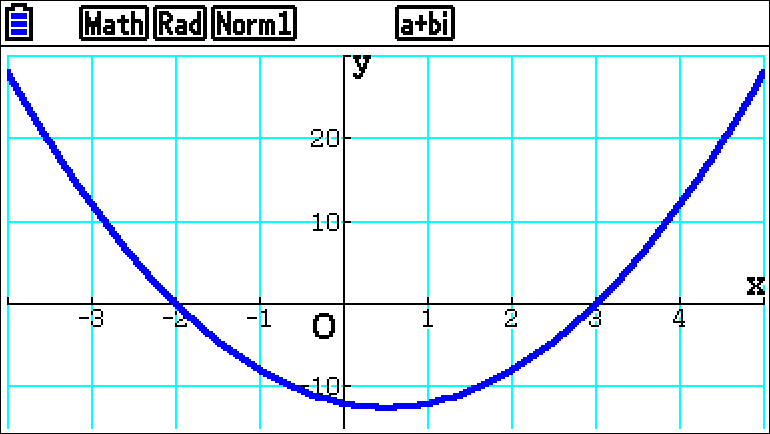
\includegraphics[width=4.5cm]{chap03_corr_exo7_a}~~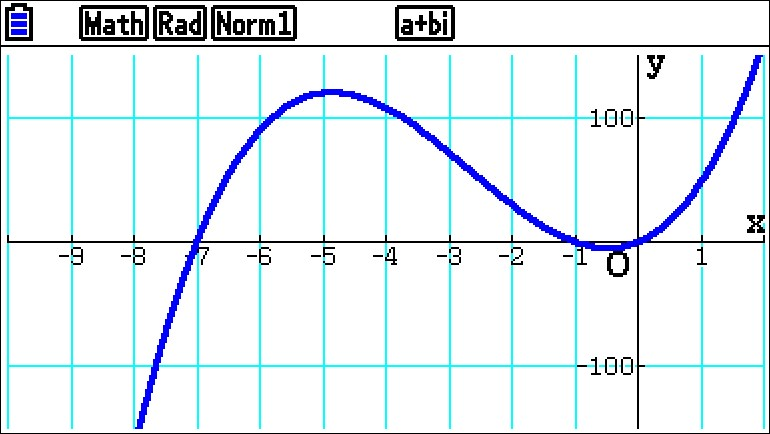
\includegraphics[width=4.5cm]{chap03_corr_exo7_b}~~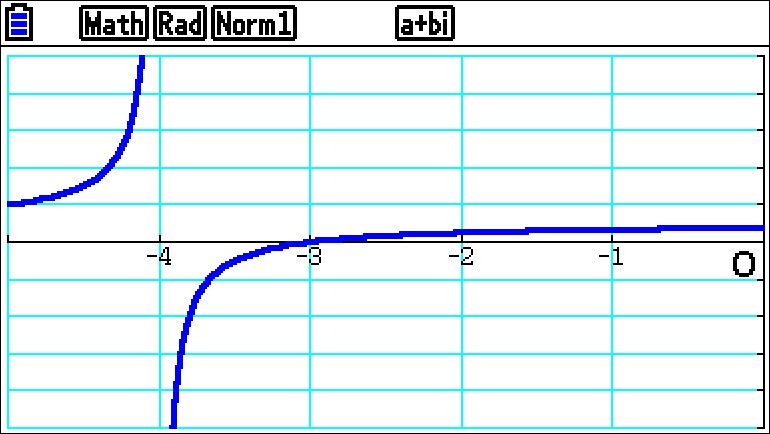
\includegraphics[width=4.5cm]{chap03_corr_exo7_c}~~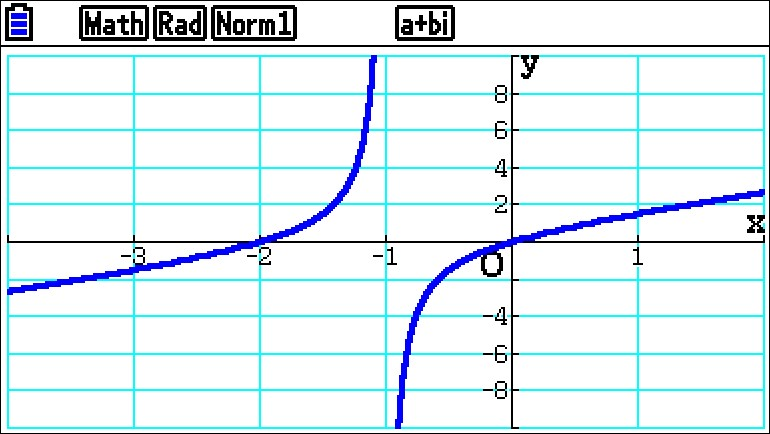
\includegraphics[width=4.5cm]{chap03_corr_exo7_d}
\end{center}
\begin{center}
	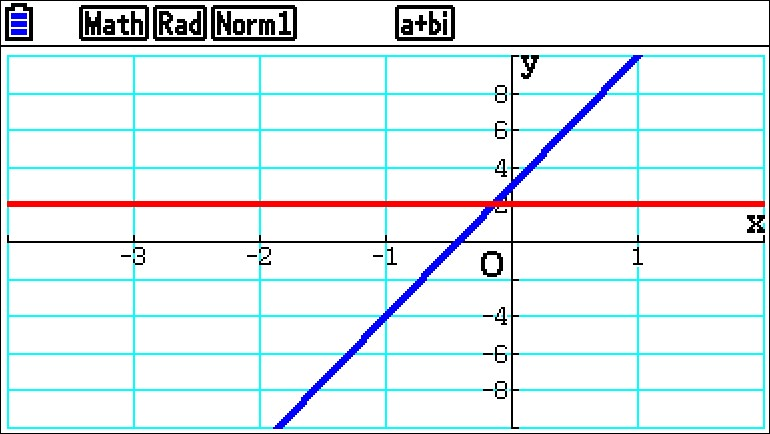
\includegraphics[width=4.5cm]{chap03_corr_exo7_e}~~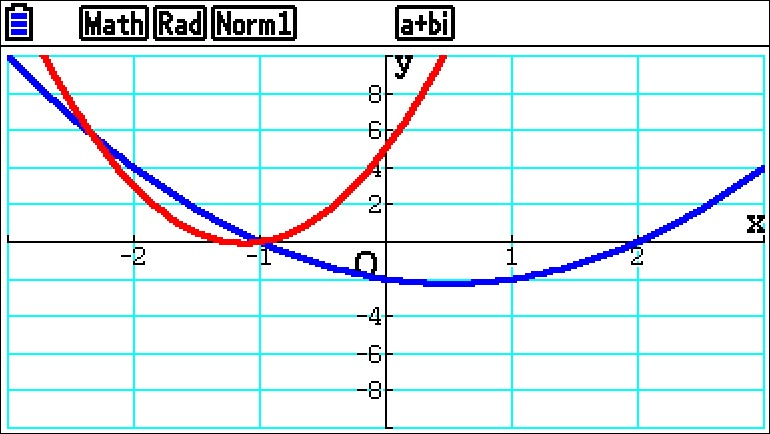
\includegraphics[width=4.5cm]{chap03_corr_exo7_f}~~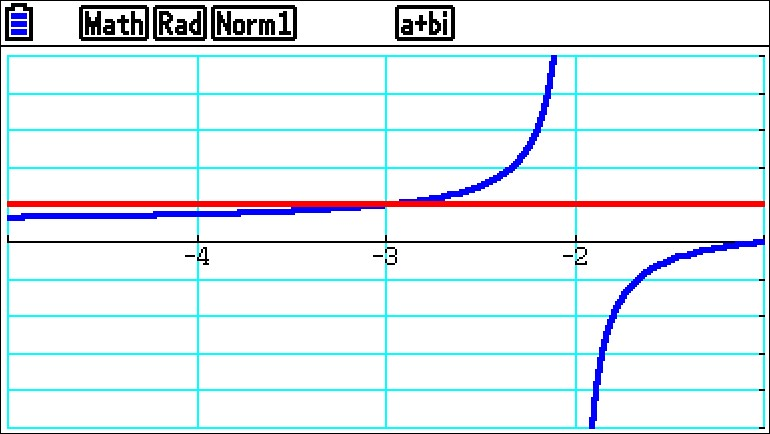
\includegraphics[width=4.5cm]{chap03_corr_exo7_g}
\end{center}

\medskip

\exonum{3}%exo8

\medskip

Le logiciel \cxcas{Xcas} nous donne les solutions de l'inéquation $\dfrac{x+5}{x+2} \pg -1$, qui sont $\intervOF{-\infty}{-\dfrac{7}{2}} \cup \intervOO{-2}{+\infty}$, en effet :

\begin{itemize}
	\item $\dfrac{x+5}{x+2} \pg 1 \ssi \dfrac{x+5}{x+2}+1 \pg 0 \ssi \dfrac{x+5}{x+2}+\dfrac{x+2}{x+2} \pg 0 \ssi \dfrac{2x+7}{x+2} \pg 0$ (\textsf{ZPQ} $\checkmark$)
	\smallskip
	\item $2x+7=0 \ssi x=-\tfrac72$ et $x+2=0 \ssi x=-2$
	
	\begin{center}
		\begin{tikzpicture}[double distance=3]
			\tkzTabInit[lgt=2.5]{$x$/0.8,$(x+5)$/0.8,$(x+2)$/0.8,expr/0.8}{$-\infty$, $\nicefrac{-7}{2}$, $-2$, $+\infty$}
			\draw[] (T21) -- (T22) node [midway, right] {$\: m=1 \: \oplus$};
			\draw[] (T22) -- (T23) node [midway, right] {$\: m=1 \: \oplus$};
			\draw(N31) node [yshift=3pt] {{\scriptsize \red \textsf{D}}};
			\tkzTabLine{,-,z,-,t,+,}
			\tkzTabLine{,-,t,+,z,+,}
			\tkzTabLine{,+,z,-,d,+,}
		\end{tikzpicture}
	\end{center}
	\begin{center}
		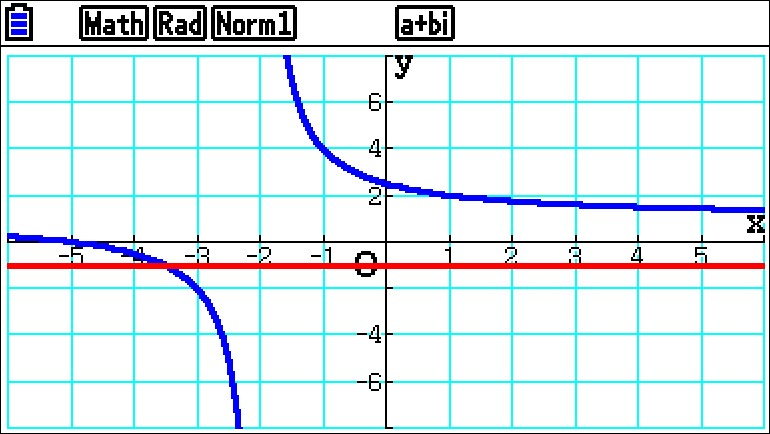
\includegraphics[width=4.5cm]{chap03_corr_exo8}
	\end{center}
\end{itemize}

\end{document}